\documentclass[1p]{elsarticle_modified}
%\bibliographystyle{elsarticle-num}

%\usepackage[colorlinks]{hyperref}
%\usepackage{abbrmath_seonhwa} %\Abb, \Ascr, \Acal ,\Abf, \Afrak
\usepackage{amsfonts}
\usepackage{amssymb}
\usepackage{amsmath}
\usepackage{amsthm}
\usepackage{scalefnt}
\usepackage{amsbsy}
\usepackage{kotex}
\usepackage{caption}
\usepackage{subfig}
\usepackage{color}
\usepackage{graphicx}
\usepackage{xcolor} %% white, black, red, green, blue, cyan, magenta, yellow
\usepackage{float}
\usepackage{setspace}
\usepackage{hyperref}

\usepackage{tikz}
\usetikzlibrary{arrows}

\usepackage{multirow}
\usepackage{array} % fixed length table
\usepackage{hhline}

%%%%%%%%%%%%%%%%%%%%%
\makeatletter
\renewcommand*\env@matrix[1][\arraystretch]{%
	\edef\arraystretch{#1}%
	\hskip -\arraycolsep
	\let\@ifnextchar\new@ifnextchar
	\array{*\c@MaxMatrixCols c}}
\makeatother %https://tex.stackexchange.com/questions/14071/how-can-i-increase-the-line-spacing-in-a-matrix
%%%%%%%%%%%%%%%

\usepackage[normalem]{ulem}

\newcommand{\msout}[1]{\ifmmode\text{\sout{\ensuremath{#1}}}\else\sout{#1}\fi}
%SOURCE: \msout is \stkout macro in https://tex.stackexchange.com/questions/20609/strikeout-in-math-mode

\newcommand{\cancel}[1]{
	\ifmmode
	{\color{red}\msout{#1}}
	\else
	{\color{red}\sout{#1}}
	\fi
}

\newcommand{\add}[1]{
	{\color{blue}\uwave{#1}}
}

\newcommand{\replace}[2]{
	\ifmmode
	{\color{red}\msout{#1}}{\color{blue}\uwave{#2}}
	\else
	{\color{red}\sout{#1}}{\color{blue}\uwave{#2}}
	\fi
}

\newcommand{\Sol}{\mathcal{S}} %segment
\newcommand{\D}{D} %diagram
\newcommand{\A}{\mathcal{A}} %arc


%%%%%%%%%%%%%%%%%%%%%%%%%%%%%5 test

\def\sl{\operatorname{\textup{SL}}(2,\Cbb)}
\def\psl{\operatorname{\textup{PSL}}(2,\Cbb)}
\def\quan{\mkern 1mu \triangleright \mkern 1mu}

\theoremstyle{definition}
\newtheorem{thm}{Theorem}[section]
\newtheorem{prop}[thm]{Proposition}
\newtheorem{lem}[thm]{Lemma}
\newtheorem{ques}[thm]{Question}
\newtheorem{cor}[thm]{Corollary}
\newtheorem{defn}[thm]{Definition}
\newtheorem{exam}[thm]{Example}
\newtheorem{rmk}[thm]{Remark}
\newtheorem{alg}[thm]{Algorithm}

\newcommand{\I}{\sqrt{-1}}
\begin{document}

%\begin{frontmatter}
%
%\title{Boundary parabolic representations of knots up to 8 crossings}
%
%%% Group authors per affiliation:
%\author{Yunhi Cho} 
%\address{Department of Mathematics, University of Seoul, Seoul, Korea}
%\ead{yhcho@uos.ac.kr}
%
%
%\author{Seonhwa Kim} %\fnref{s_kim}}
%\address{Center for Geometry and Physics, Institute for Basic Science, Pohang, 37673, Korea}
%\ead{ryeona17@ibs.re.kr}
%
%\author{Hyuk Kim}
%\address{Department of Mathematical Sciences, Seoul National University, Seoul 08826, Korea}
%\ead{hyukkim@snu.ac.kr}
%
%\author{Seokbeom Yoon}
%\address{Department of Mathematical Sciences, Seoul National University, Seoul, 08826,  Korea}
%\ead{sbyoon15@snu.ac.kr}
%
%\begin{abstract}
%We find all boundary parabolic representation of knots up to 8 crossings.
%
%\end{abstract}
%\begin{keyword}
%    \MSC[2010] 57M25 
%\end{keyword}
%
%\end{frontmatter}

%\linenumbers
%\tableofcontents
%
\newcommand\colored[1]{\textcolor{white}{\rule[-0.35ex]{0.8em}{1.4ex}}\kern-0.8em\color{red} #1}%
%\newcommand\colored[1]{\textcolor{white}{ #1}\kern-2.17ex	\textcolor{white}{ #1}\kern-1.81ex	\textcolor{white}{ #1}\kern-2.15ex\color{red}#1	}

{\Large $\underline{12n_{0060}~(K12n_{0060})}$}

\setlength{\tabcolsep}{10pt}
\renewcommand{\arraystretch}{1.6}
\vspace{1cm}\begin{tabular}{m{100pt}>{\centering\arraybackslash}m{274pt}}
\multirow{5}{120pt}{
	\centering
	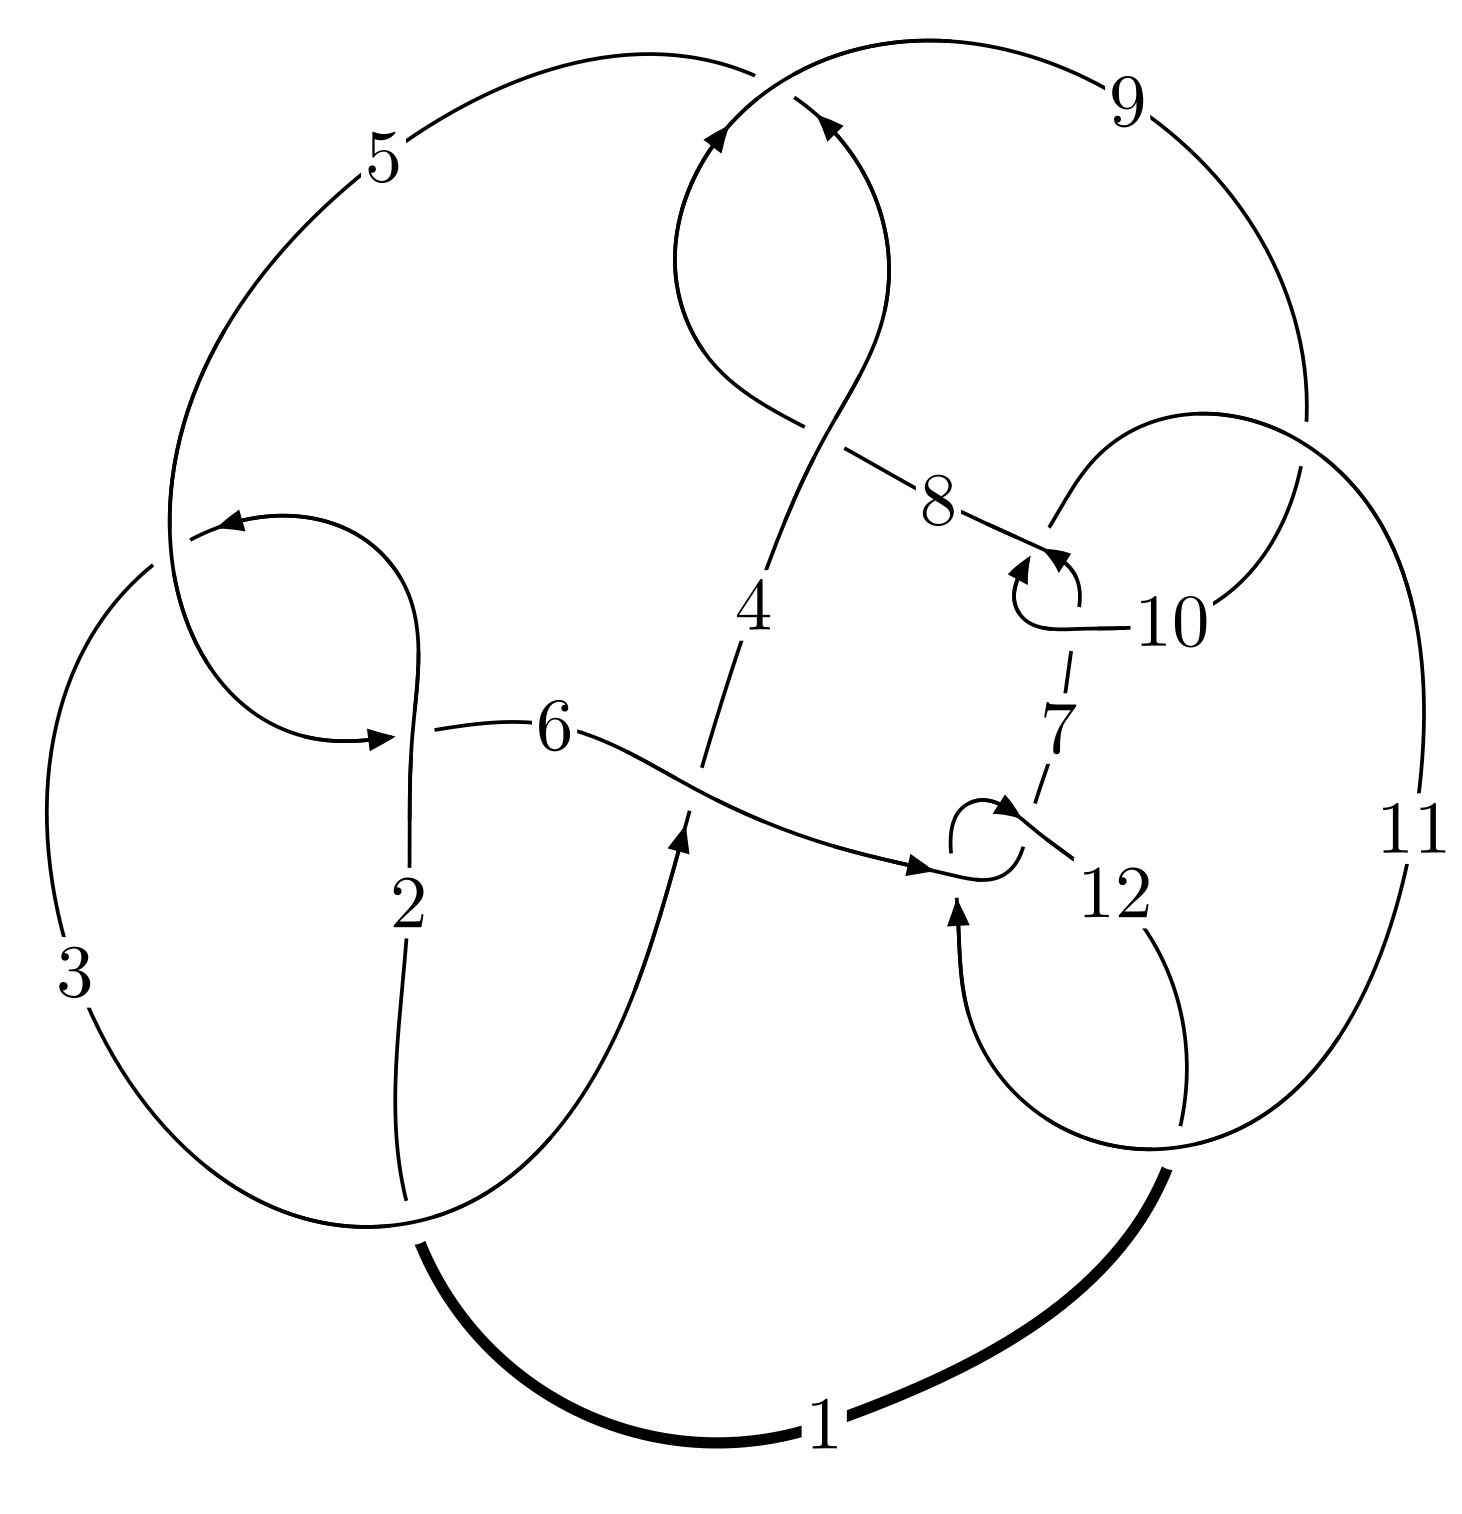
\includegraphics[width=112pt]{../../../GIT/diagram.site/Diagrams/png/2149_12n_0060.png}\\
\ \ \ A knot diagram\footnotemark}&
\allowdisplaybreaks
\textbf{Linearized knot diagam} \\
\cline{2-2}
 &
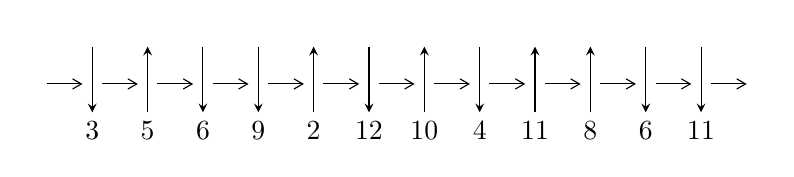
\begin{tikzpicture}[x=20pt, y=17pt]
	% nodes
	\node (C0) at (0, 0) {};
	\node (C1) at (1, 0) {};
	\node (C1U) at (1, +1) {};
	\node (C1D) at (1, -1) {3};

	\node (C2) at (2, 0) {};
	\node (C2U) at (2, +1) {};
	\node (C2D) at (2, -1) {5};

	\node (C3) at (3, 0) {};
	\node (C3U) at (3, +1) {};
	\node (C3D) at (3, -1) {6};

	\node (C4) at (4, 0) {};
	\node (C4U) at (4, +1) {};
	\node (C4D) at (4, -1) {9};

	\node (C5) at (5, 0) {};
	\node (C5U) at (5, +1) {};
	\node (C5D) at (5, -1) {2};

	\node (C6) at (6, 0) {};
	\node (C6U) at (6, +1) {};
	\node (C6D) at (6, -1) {12};

	\node (C7) at (7, 0) {};
	\node (C7U) at (7, +1) {};
	\node (C7D) at (7, -1) {10};

	\node (C8) at (8, 0) {};
	\node (C8U) at (8, +1) {};
	\node (C8D) at (8, -1) {4};

	\node (C9) at (9, 0) {};
	\node (C9U) at (9, +1) {};
	\node (C9D) at (9, -1) {11};

	\node (C10) at (10, 0) {};
	\node (C10U) at (10, +1) {};
	\node (C10D) at (10, -1) {8};

	\node (C11) at (11, 0) {};
	\node (C11U) at (11, +1) {};
	\node (C11D) at (11, -1) {6};

	\node (C12) at (12, 0) {};
	\node (C12U) at (12, +1) {};
	\node (C12D) at (12, -1) {11};
	\node (C13) at (13, 0) {};

	% arrows
	\draw[->,>={angle 60}]
	(C0) edge (C1) (C1) edge (C2) (C2) edge (C3) (C3) edge (C4) (C4) edge (C5) (C5) edge (C6) (C6) edge (C7) (C7) edge (C8) (C8) edge (C9) (C9) edge (C10) (C10) edge (C11) (C11) edge (C12) (C12) edge (C13) ;	\draw[->,>=stealth]
	(C1U) edge (C1D) (C2D) edge (C2U) (C3U) edge (C3D) (C4U) edge (C4D) (C5D) edge (C5U) (C6U) edge (C6D) (C7D) edge (C7U) (C8U) edge (C8D) (C9D) edge (C9U) (C10D) edge (C10U) (C11U) edge (C11D) (C12U) edge (C12D) ;
	\end{tikzpicture} \\
\hhline{~~} \\& 
\textbf{Solving Sequence} \\ \cline{2-2} 
 &
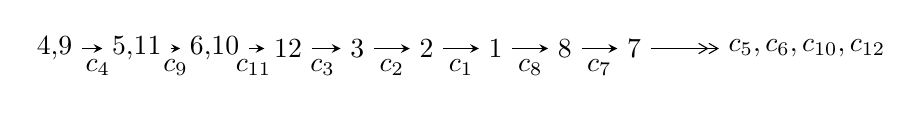
\begin{tikzpicture}[x=25pt, y=7pt]
	% node
	\node (A0) at (-1/8, 0) {4,9};
	\node (A1) at (17/16, 0) {5,11};
	\node (A2) at (35/16, 0) {6,10};
	\node (A3) at (13/4, 0) {12};
	\node (A4) at (17/4, 0) {3};
	\node (A5) at (21/4, 0) {2};
	\node (A6) at (25/4, 0) {1};
	\node (A7) at (29/4, 0) {8};
	\node (A8) at (33/4, 0) {7};
	\node (C1) at (1/2, -1) {$c_{4}$};
	\node (C2) at (13/8, -1) {$c_{9}$};
	\node (C3) at (11/4, -1) {$c_{11}$};
	\node (C4) at (15/4, -1) {$c_{3}$};
	\node (C5) at (19/4, -1) {$c_{2}$};
	\node (C6) at (23/4, -1) {$c_{1}$};
	\node (C7) at (27/4, -1) {$c_{8}$};
	\node (C8) at (31/4, -1) {$c_{7}$};
	\node (A9) at (43/4, 0) {$c_{5},c_{6},c_{10},c_{12}$};

	% edge
	\draw[->,>=stealth]	
	(A0) edge (A1) (A1) edge (A2) (A2) edge (A3) (A3) edge (A4) (A4) edge (A5) (A5) edge (A6) (A6) edge (A7) (A7) edge (A8) ;
	\draw[->>,>={angle 60}]	
	(A8) edge (A9);
\end{tikzpicture} \\ 

\end{tabular} \\

\footnotetext{
The image of knot diagram is generated by the software ``\textbf{Draw programme}" developed by Andrew Bartholomew(\url{http://www.layer8.co.uk/maths/draw/index.htm\#Running-draw}), where we modified some parts for our purpose(\url{https://github.com/CATsTAILs/LinksPainter}).
}\phantom \\ \newline 
\centering \textbf{Ideals for irreducible components\footnotemark of $X_{\text{par}}$} 
 
\begin{align*}
I^u_{1}&=\langle 
-2.71438\times10^{84} u^{46}-3.94862\times10^{84} u^{45}+\cdots+5.11546\times10^{87} d+5.51326\times10^{87},\\
\phantom{I^u_{1}}&\phantom{= \langle  }1.81915\times10^{85} u^{46}-2.40556\times10^{85} u^{45}+\cdots+1.27887\times10^{87} c+1.47462\times10^{88},\\
\phantom{I^u_{1}}&\phantom{= \langle  }-7.84763\times10^{95} u^{46}+5.19621\times10^{95} u^{45}+\cdots+6.09681\times10^{98} b-4.85317\times10^{98},\\
\phantom{I^u_{1}}&\phantom{= \langle  }-1.61790\times10^{97} u^{46}+2.28917\times10^{97} u^{45}+\cdots+6.09681\times10^{98} a-1.26868\times10^{100},\\
\phantom{I^u_{1}}&\phantom{= \langle  }u^{47}-2 u^{46}+\cdots+1024 u-512\rangle \\
I^u_{2}&=\langle 
u^4 c^2+u^3 c^2- u^4 c-2 c^2 u^2-2 u^3 c- c^2 u+u^2 c+c^2+3 c u+d- c,\\
\phantom{I^u_{2}}&\phantom{= \langle  }-2 u^4 c^2-2 u^3 c^2+u^4 c+4 c^2 u^2+2 u^3 c+c^3+2 c^2 u- u^2 c-2 c^2-3 c u- u,\;b- u,\;a- u,\\
\phantom{I^u_{2}}&\phantom{= \langle  }u^5+u^4-2 u^3- u^2+u-1\rangle \\
\\
I^v_{1}&=\langle 
a,\;d- v+1,\;c+a,\;b+v-1,\;v^2- v+1\rangle \\
I^v_{2}&=\langle 
a,\;d,\;c- v,\;b- v-1,\;v^2+v+1\rangle \\
I^v_{3}&=\langle 
c,\;d+1,\;b,\;a-1,\;v-1\rangle \\
I^v_{4}&=\langle 
a,\;d a- c b+1,\;d v+1,\;c v- b a+b v+a- v,\;b^2- b+1\rangle \\
\end{align*}
\raggedright * 5 irreducible components of $\dim_{\mathbb{C}}=0$, with total 67 representations.\\
\raggedright * 1 irreducible components of $\dim_{\mathbb{C}}=1$ \\
\footnotetext{All coefficients of polynomials are rational numbers. But the coefficients are sometimes approximated in decimal forms when there is not enough margin.}
\newpage
\renewcommand{\arraystretch}{1}
\centering \section*{I. $I^u_{1}= \langle -2.71\times10^{84} u^{46}-3.95\times10^{84} u^{45}+\cdots+5.12\times10^{87} d+5.51\times10^{87},\;1.82\times10^{85} u^{46}-2.41\times10^{85} u^{45}+\cdots+1.28\times10^{87} c+1.47\times10^{88},\;-7.85\times10^{95} u^{46}+5.20\times10^{95} u^{45}+\cdots+6.10\times10^{98} b-4.85\times10^{98},\;-1.62\times10^{97} u^{46}+2.29\times10^{97} u^{45}+\cdots+6.10\times10^{98} a-1.27\times10^{100},\;u^{47}-2 u^{46}+\cdots+1024 u-512 \rangle$}
\flushleft \textbf{(i) Arc colorings}\\
\begin{tabular}{m{7pt} m{180pt} m{7pt} m{180pt} }
\flushright $a_{4}=$&$\begin{pmatrix}1\\0\end{pmatrix}$ \\
\flushright $a_{9}=$&$\begin{pmatrix}0\\u\end{pmatrix}$ \\
\flushright $a_{5}=$&$\begin{pmatrix}1\\u^2\end{pmatrix}$ \\
\flushright $a_{11}=$&$\begin{pmatrix}-0.0142247 u^{46}+0.0188101 u^{45}+\cdots+6.02241 u-11.5307\\0.000530623 u^{46}+0.000771899 u^{45}+\cdots-0.720071 u-1.07776\end{pmatrix}$ \\
\flushright $a_{6}=$&$\begin{pmatrix}0.0265369 u^{46}-0.0375470 u^{45}+\cdots-11.6287 u+20.8089\\0.00128717 u^{46}-0.000852284 u^{45}+\cdots-0.317834 u+0.796018\end{pmatrix}$ \\
\flushright $a_{10}=$&$\begin{pmatrix}-0.0226340 u^{46}+0.0298604 u^{45}+\cdots+10.2154 u-17.4046\\-0.00787872 u^{46}+0.0118222 u^{45}+\cdots+3.47297 u-6.95164\end{pmatrix}$ \\
\flushright $a_{12}=$&$\begin{pmatrix}-0.0239734 u^{46}+0.0351954 u^{45}+\cdots+10.0932 u-19.6370\\-0.000874062 u^{46}+0.00264928 u^{45}+\cdots-0.431382 u-2.36213\end{pmatrix}$ \\
\flushright $a_{3}=$&$\begin{pmatrix}0.00513208 u^{46}-0.00817440 u^{45}+\cdots+0.763266 u+5.03316\\0.00862965 u^{46}-0.0123123 u^{45}+\cdots-4.96716 u+7.59297\end{pmatrix}$ \\
\flushright $a_{2}=$&$\begin{pmatrix}-0.00521744 u^{46}+0.00448641 u^{45}+\cdots+6.21813 u-1.48986\\0.00291266 u^{46}-0.00502319 u^{45}+\cdots-2.03496 u+3.47740\end{pmatrix}$ \\
\flushright $a_{1}=$&$\begin{pmatrix}0.0252497 u^{46}-0.0366947 u^{45}+\cdots-11.3108 u+20.0129\\0.00558802 u^{46}-0.00914935 u^{45}+\cdots-0.890394 u+6.27203\end{pmatrix}$ \\
\flushright $a_{8}=$&$\begin{pmatrix}u\\u\end{pmatrix}$ \\
\flushright $a_{7}=$&$\begin{pmatrix}0.0207800 u^{46}-0.0264941 u^{45}+\cdots-9.33005 u+15.3882\\0.00655528 u^{46}-0.00768405 u^{45}+\cdots-3.30765 u+3.85754\end{pmatrix}$\\&\end{tabular}
\flushleft \textbf{(ii) Obstruction class $= -1$}\\~\\
\flushleft \textbf{(iii) Cusp Shapes $= 0.0132573 u^{46}-0.0100723 u^{45}+\cdots-23.2337 u-1.69873$}\\~\\
\newpage\renewcommand{\arraystretch}{1}
\flushleft \textbf{(iv) u-Polynomials at the component}\newline \\
\begin{tabular}{m{50pt}|m{274pt}}
Crossings & \hspace{64pt}u-Polynomials at each crossing \\
\hline $$\begin{aligned}c_{1}\end{aligned}$$&$\begin{aligned}
&u^{47}+24 u^{46}+\cdots+216 u-16
\end{aligned}$\\
\hline $$\begin{aligned}c_{2},c_{5}\end{aligned}$$&$\begin{aligned}
&u^{47}+2 u^{46}+\cdots+16 u+4
\end{aligned}$\\
\hline $$\begin{aligned}c_{3}\end{aligned}$$&$\begin{aligned}
&u^{47}-2 u^{46}+\cdots-21456 u+2592
\end{aligned}$\\
\hline $$\begin{aligned}c_{4},c_{8}\end{aligned}$$&$\begin{aligned}
&u^{47}+2 u^{46}+\cdots+1024 u+512
\end{aligned}$\\
\hline $$\begin{aligned}c_{6},c_{11}\end{aligned}$$&$\begin{aligned}
&u^{47}-8 u^{46}+\cdots+56 u+16
\end{aligned}$\\
\hline $$\begin{aligned}c_{7},c_{10}\end{aligned}$$&$\begin{aligned}
&u^{47}+8 u^{46}+\cdots+56 u+16
\end{aligned}$\\
\hline $$\begin{aligned}c_{9}\end{aligned}$$&$\begin{aligned}
&u^{47}-14 u^{46}+\cdots+6688 u-256
\end{aligned}$\\
\hline $$\begin{aligned}c_{12}\end{aligned}$$&$\begin{aligned}
&u^{47}+54 u^{46}+\cdots+544 u+256
\end{aligned}$\\
\hline
\end{tabular}\\~\\
\newpage\renewcommand{\arraystretch}{1}
\flushleft \textbf{(v) Riley Polynomials at the component}\newline \\
\begin{tabular}{m{50pt}|m{274pt}}
Crossings & \hspace{64pt}Riley Polynomials at each crossing \\
\hline $$\begin{aligned}c_{1}\end{aligned}$$&$\begin{aligned}
&y^{47}+48 y^{45}+\cdots+67872 y-256
\end{aligned}$\\
\hline $$\begin{aligned}c_{2},c_{5}\end{aligned}$$&$\begin{aligned}
&y^{47}+24 y^{46}+\cdots+216 y-16
\end{aligned}$\\
\hline $$\begin{aligned}c_{3}\end{aligned}$$&$\begin{aligned}
&y^{47}-24 y^{46}+\cdots+353776896 y-6718464
\end{aligned}$\\
\hline $$\begin{aligned}c_{4},c_{8}\end{aligned}$$&$\begin{aligned}
&y^{47}-30 y^{46}+\cdots+1572864 y-262144
\end{aligned}$\\
\hline $$\begin{aligned}c_{6},c_{11}\end{aligned}$$&$\begin{aligned}
&y^{47}-54 y^{46}+\cdots+544 y-256
\end{aligned}$\\
\hline $$\begin{aligned}c_{7},c_{10}\end{aligned}$$&$\begin{aligned}
&y^{47}-14 y^{46}+\cdots+6688 y-256
\end{aligned}$\\
\hline $$\begin{aligned}c_{9}\end{aligned}$$&$\begin{aligned}
&y^{47}+46 y^{46}+\cdots+11182592 y-65536
\end{aligned}$\\
\hline $$\begin{aligned}c_{12}\end{aligned}$$&$\begin{aligned}
&y^{47}-114 y^{46}+\cdots-1990144 y-65536
\end{aligned}$\\
\hline
\end{tabular}\\~\\
\newpage\flushleft \textbf{(vi) Complex Volumes and Cusp Shapes}
$$\begin{array}{c|c|c}  
\text{Solutions to }I^u_{1}& \I (\text{vol} + \sqrt{-1}CS) & \text{Cusp shape}\\
 \hline 
\begin{aligned}
u &= \phantom{-}0.168857 + 0.977277 I \\
a &= \phantom{-}0.115176 - 0.466477 I \\
b &= \phantom{-}0.993069 - 0.480924 I \\
c &= \phantom{-}0.880204 - 0.225891 I \\
d &= \phantom{-}0.230994 + 0.477533 I\end{aligned}
 & -0.50019 + 4.79223 I & -2.43501 - 7.48976 I \\ \hline\begin{aligned}
u &= \phantom{-}0.168857 - 0.977277 I \\
a &= \phantom{-}0.115176 + 0.466477 I \\
b &= \phantom{-}0.993069 + 0.480924 I \\
c &= \phantom{-}0.880204 + 0.225891 I \\
d &= \phantom{-}0.230994 - 0.477533 I\end{aligned}
 & -0.50019 - 4.79223 I & -2.43501 + 7.48976 I \\ \hline\begin{aligned}
u &= -0.758370 + 0.572620 I \\
a &= -0.056911 - 1.268310 I \\
b &= -0.176331 - 0.077095 I \\
c &= \phantom{-}0.238166 + 0.368256 I \\
d &= -0.259334 + 0.830862 I\end{aligned}
 & -3.62778 - 1.19000 I & -10.45074 + 1.01195 I \\ \hline\begin{aligned}
u &= -0.758370 - 0.572620 I \\
a &= -0.056911 + 1.268310 I \\
b &= -0.176331 + 0.077095 I \\
c &= \phantom{-}0.238166 - 0.368256 I \\
d &= -0.259334 - 0.830862 I\end{aligned}
 & -3.62778 + 1.19000 I & -10.45074 - 1.01195 I \\ \hline\begin{aligned}
u &= -0.798854 + 0.256222 I \\
a &= \phantom{-}0.287839 - 0.327673 I \\
b &= \phantom{-}0.167965 - 1.279390 I \\
c &= -0.461116 - 0.948349 I \\
d &= -1.30820 - 1.68280 I\end{aligned}
 & \phantom{-}1.43042 + 3.68269 I & -0.57615 - 8.67104 I \\ \hline\begin{aligned}
u &= -0.798854 - 0.256222 I \\
a &= \phantom{-}0.287839 + 0.327673 I \\
b &= \phantom{-}0.167965 + 1.279390 I \\
c &= -0.461116 + 0.948349 I \\
d &= -1.30820 + 1.68280 I\end{aligned}
 & \phantom{-}1.43042 - 3.68269 I & -0.57615 + 8.67104 I\\
 \hline 
 \end{array}$$\newpage$$\begin{array}{c|c|c}  
\text{Solutions to }I^u_{1}& \I (\text{vol} + \sqrt{-1}CS) & \text{Cusp shape}\\
 \hline 
\begin{aligned}
u &= -0.287114 + 0.709757 I \\
a &= \phantom{-}0.578531 - 0.174810 I \\
b &= -0.451429 - 0.388165 I \\
c &= -1.015380 - 0.600162 I \\
d &= -0.205691 + 0.340554 I\end{aligned}
 & \phantom{-}1.71355 - 0.99880 I & \phantom{-}4.04476 + 2.43406 I \\ \hline\begin{aligned}
u &= -0.287114 - 0.709757 I \\
a &= \phantom{-}0.578531 + 0.174810 I \\
b &= -0.451429 + 0.388165 I \\
c &= -1.015380 + 0.600162 I \\
d &= -0.205691 - 0.340554 I\end{aligned}
 & \phantom{-}1.71355 + 0.99880 I & \phantom{-}4.04476 - 2.43406 I \\ \hline\begin{aligned}
u &= \phantom{-}0.723521 + 0.092490 I \\
a &= -3.48927 - 1.92959 I \\
b &= -0.757487 - 0.595429 I \\
c &= \phantom{-}1.96585 - 0.11713 I \\
d &= \phantom{-}0.329861 + 0.036001 I\end{aligned}
 & \phantom{-}0.84436 - 2.80891 I & -4.36866 + 6.45196 I \\ \hline\begin{aligned}
u &= \phantom{-}0.723521 - 0.092490 I \\
a &= -3.48927 + 1.92959 I \\
b &= -0.757487 + 0.595429 I \\
c &= \phantom{-}1.96585 + 0.11713 I \\
d &= \phantom{-}0.329861 - 0.036001 I\end{aligned}
 & \phantom{-}0.84436 + 2.80891 I & -4.36866 - 6.45196 I \\ \hline\begin{aligned}
u &= -0.549584 + 0.433005 I \\
a &= \phantom{-}1.88335 - 0.62690 I \\
b &= \phantom{-}0.086194 - 0.585488 I \\
c &= -1.67372 - 0.58265 I \\
d &= -0.277903 + 0.181976 I\end{aligned}
 & \phantom{-}2.18982 - 0.74670 I & \phantom{-}2.91211 - 1.96105 I \\ \hline\begin{aligned}
u &= -0.549584 - 0.433005 I \\
a &= \phantom{-}1.88335 + 0.62690 I \\
b &= \phantom{-}0.086194 + 0.585488 I \\
c &= -1.67372 + 0.58265 I \\
d &= -0.277903 - 0.181976 I\end{aligned}
 & \phantom{-}2.18982 + 0.74670 I & \phantom{-}2.91211 + 1.96105 I\\
 \hline 
 \end{array}$$\newpage$$\begin{array}{c|c|c}  
\text{Solutions to }I^u_{1}& \I (\text{vol} + \sqrt{-1}CS) & \text{Cusp shape}\\
 \hline 
\begin{aligned}
u &= \phantom{-}0.659997 + 0.157577 I \\
a &= \phantom{-}0.229959 - 0.371748 I \\
b &= \phantom{-}0.575360 - 1.171710 I \\
c &= \phantom{-}0.729227 - 0.739183 I \\
d &= \phantom{-}1.80686 - 1.34660 I\end{aligned}
 & \phantom{-}1.05099 + 1.22135 I & -3.11104 + 2.86511 I \\ \hline\begin{aligned}
u &= \phantom{-}0.659997 - 0.157577 I \\
a &= \phantom{-}0.229959 + 0.371748 I \\
b &= \phantom{-}0.575360 + 1.171710 I \\
c &= \phantom{-}0.729227 + 0.739183 I \\
d &= \phantom{-}1.80686 + 1.34660 I\end{aligned}
 & \phantom{-}1.05099 - 1.22135 I & -3.11104 - 2.86511 I \\ \hline\begin{aligned}
u &= \phantom{-}0.226818 + 1.310000 I \\
a &= \phantom{-}0.395536 + 0.047557 I \\
b &= -1.354130 + 0.342438 I \\
c &= \phantom{-}1.007050 - 0.000849 I \\
d &= \phantom{-}0.341442 + 0.559896 I\end{aligned}
 & -4.12204 + 2.83071 I & -3.10594 - 2.47522 I \\ \hline\begin{aligned}
u &= \phantom{-}0.226818 - 1.310000 I \\
a &= \phantom{-}0.395536 - 0.047557 I \\
b &= -1.354130 - 0.342438 I \\
c &= \phantom{-}1.007050 + 0.000849 I \\
d &= \phantom{-}0.341442 - 0.559896 I\end{aligned}
 & -4.12204 - 2.83071 I & -3.10594 + 2.47522 I \\ \hline\begin{aligned}
u &= -0.024914 + 0.666306 I \\
a &= \phantom{-}0.187765 + 0.490307 I \\
b &= \phantom{-}0.676859 + 0.593604 I \\
c &= \phantom{-}0.299606 - 0.388234 I \\
d &= \phantom{-}0.038036 + 0.428504 I\end{aligned}
 & -0.68586 - 1.51893 I & -2.03699 - 0.09471 I \\ \hline\begin{aligned}
u &= -0.024914 - 0.666306 I \\
a &= \phantom{-}0.187765 - 0.490307 I \\
b &= \phantom{-}0.676859 - 0.593604 I \\
c &= \phantom{-}0.299606 + 0.388234 I \\
d &= \phantom{-}0.038036 - 0.428504 I\end{aligned}
 & -0.68586 + 1.51893 I & -2.03699 + 0.09471 I\\
 \hline 
 \end{array}$$\newpage$$\begin{array}{c|c|c}  
\text{Solutions to }I^u_{1}& \I (\text{vol} + \sqrt{-1}CS) & \text{Cusp shape}\\
 \hline 
\begin{aligned}
u &= -1.275400 + 0.425723 I \\
a &= \phantom{-}1.190730 + 0.205684 I \\
b &= \phantom{-}1.29665 - 0.64292 I \\
c &= -0.045370 - 1.113460 I \\
d &= -0.59246 - 1.84112 I\end{aligned}
 & -1.49383 + 5.48046 I & -1.24533 - 5.03878 I \\ \hline\begin{aligned}
u &= -1.275400 - 0.425723 I \\
a &= \phantom{-}1.190730 - 0.205684 I \\
b &= \phantom{-}1.29665 + 0.64292 I \\
c &= -0.045370 + 1.113460 I \\
d &= -0.59246 + 1.84112 I\end{aligned}
 & -1.49383 - 5.48046 I & -1.24533 + 5.03878 I \\ \hline\begin{aligned}
u &= -1.351470 + 0.126259 I \\
a &= \phantom{-}0.200409 + 0.288465 I \\
b &= \phantom{-}0.63511 + 1.89146 I \\
c &= \phantom{-}0.044710 - 0.963693 I \\
d &= -0.50842 - 1.59992 I\end{aligned}
 & -5.10242 - 0.08441 I & -6.12902 + 0. I\phantom{ +0.000000I} \\ \hline\begin{aligned}
u &= -1.351470 - 0.126259 I \\
a &= \phantom{-}0.200409 - 0.288465 I \\
b &= \phantom{-}0.63511 - 1.89146 I \\
c &= \phantom{-}0.044710 + 0.963693 I \\
d &= -0.50842 + 1.59992 I\end{aligned}
 & -5.10242 + 0.08441 I & -6.12902 + 0. I\phantom{ +0.000000I} \\ \hline\begin{aligned}
u &= \phantom{-}0.062543 + 0.611080 I \\
a &= \phantom{-}2.98020 - 5.04065 I \\
b &= -0.392543 + 1.124120 I \\
c &= \phantom{-}0.382597 - 0.828016 I \\
d &= \phantom{-}0.060601 + 0.347239 I\end{aligned}
 & -0.53961 + 2.33649 I & -0.16377 - 3.97632 I \\ \hline\begin{aligned}
u &= \phantom{-}0.062543 - 0.611080 I \\
a &= \phantom{-}2.98020 + 5.04065 I \\
b &= -0.392543 - 1.124120 I \\
c &= \phantom{-}0.382597 + 0.828016 I \\
d &= \phantom{-}0.060601 - 0.347239 I\end{aligned}
 & -0.53961 - 2.33649 I & -0.16377 + 3.97632 I\\
 \hline 
 \end{array}$$\newpage$$\begin{array}{c|c|c}  
\text{Solutions to }I^u_{1}& \I (\text{vol} + \sqrt{-1}CS) & \text{Cusp shape}\\
 \hline 
\begin{aligned}
u &= \phantom{-}1.354510 + 0.305217 I \\
a &= \phantom{-}0.237962 + 0.257635 I \\
b &= \phantom{-}0.10673 + 1.95842 I \\
c &= -0.009355 - 1.056680 I \\
d &= \phantom{-}0.53250 - 1.74040 I\end{aligned}
 & -4.74548 - 5.93381 I & -5.07129 + 5.57342 I \\ \hline\begin{aligned}
u &= \phantom{-}1.354510 - 0.305217 I \\
a &= \phantom{-}0.237962 - 0.257635 I \\
b &= \phantom{-}0.10673 - 1.95842 I \\
c &= -0.009355 + 1.056680 I \\
d &= \phantom{-}0.53250 + 1.74040 I\end{aligned}
 & -4.74548 + 5.93381 I & -5.07129 - 5.57342 I \\ \hline\begin{aligned}
u &= \phantom{-}1.42975 + 0.19774 I \\
a &= -1.065100 + 0.614192 I \\
b &= -1.111480 - 0.181975 I \\
c &= -0.065967 - 1.017040 I \\
d &= \phantom{-}0.46521 - 1.66816 I\end{aligned}
 & -5.91128 - 1.72117 I & -6.79419 + 0. I\phantom{ +0.000000I} \\ \hline\begin{aligned}
u &= \phantom{-}1.42975 - 0.19774 I \\
a &= -1.065100 - 0.614192 I \\
b &= -1.111480 + 0.181975 I \\
c &= -0.065967 + 1.017040 I \\
d &= \phantom{-}0.46521 + 1.66816 I\end{aligned}
 & -5.91128 + 1.72117 I & -6.79419 + 0. I\phantom{ +0.000000I} \\ \hline\begin{aligned}
u &= \phantom{-}0.01170 + 1.48787 I \\
a &= \phantom{-}0.011715 - 0.454077 I \\
b &= \phantom{-}1.331480 + 0.029628 I \\
c &= -0.940701 + 0.145408 I \\
d &= -0.335520 + 0.668373 I\end{aligned}
 & -8.14593 + 1.35024 I & \phantom{-0.000000 } 0 \\ \hline\begin{aligned}
u &= \phantom{-}0.01170 - 1.48787 I \\
a &= \phantom{-}0.011715 + 0.454077 I \\
b &= \phantom{-}1.331480 - 0.029628 I \\
c &= -0.940701 - 0.145408 I \\
d &= -0.335520 - 0.668373 I\end{aligned}
 & -8.14593 - 1.35024 I & \phantom{-0.000000 } 0\\
 \hline 
 \end{array}$$\newpage$$\begin{array}{c|c|c}  
\text{Solutions to }I^u_{1}& \I (\text{vol} + \sqrt{-1}CS) & \text{Cusp shape}\\
 \hline 
\begin{aligned}
u &= \phantom{-}0.509235\phantom{ +0.000000I} \\
a &= \phantom{-}1.22614\phantom{ +0.000000I} \\
b &= \phantom{-}0.258456\phantom{ +0.000000I} \\
c &= \phantom{-}0.155794\phantom{ +0.000000I} \\
d &= \phantom{-}0.708911\phantom{ +0.000000I}\end{aligned}
 & -1.19981\phantom{ +0.000000I} & -8.75910\phantom{ +0.000000I} \\ \hline\begin{aligned}
u &= \phantom{-}1.38697 + 0.55724 I \\
a &= -1.46233 + 0.24224 I \\
b &= -1.61416 - 0.56868 I \\
c &= -0.006312 - 1.182540 I \\
d &= \phantom{-}0.48982 - 1.92078 I\end{aligned}
 & -4.40802 - 10.56830 I & \phantom{-0.000000 } 0 \\ \hline\begin{aligned}
u &= \phantom{-}1.38697 - 0.55724 I \\
a &= -1.46233 - 0.24224 I \\
b &= -1.61416 + 0.56868 I \\
c &= -0.006312 + 1.182540 I \\
d &= \phantom{-}0.48982 + 1.92078 I\end{aligned}
 & -4.40802 + 10.56830 I & \phantom{-0.000000 } 0 \\ \hline\begin{aligned}
u &= -0.40359 + 1.45989 I \\
a &= \phantom{-}0.049725 + 0.404703 I \\
b &= \phantom{-}1.58609 + 0.36933 I \\
c &= -1.117100 + 0.048331 I \\
d &= -0.422301 + 0.553774 I\end{aligned}
 & -7.37650 - 7.69255 I & \phantom{-0.000000 } 0 \\ \hline\begin{aligned}
u &= -0.40359 - 1.45989 I \\
a &= \phantom{-}0.049725 - 0.404703 I \\
b &= \phantom{-}1.58609 - 0.36933 I \\
c &= -1.117100 - 0.048331 I \\
d &= -0.422301 - 0.553774 I\end{aligned}
 & -7.37650 + 7.69255 I & \phantom{-0.000000 } 0 \\ \hline\begin{aligned}
u &= \phantom{-}1.43182 + 0.71566 I \\
a &= \phantom{-}1.063460 - 0.335902 I \\
b &= \phantom{-}1.52462 + 1.08887 I \\
c &= -0.026296 - 1.248550 I \\
d &= \phantom{-}0.43018 - 2.00472 I\end{aligned}
 & -7.91018 - 10.04820 I & \phantom{-0.000000 } 0\\
 \hline 
 \end{array}$$\newpage$$\begin{array}{c|c|c}  
\text{Solutions to }I^u_{1}& \I (\text{vol} + \sqrt{-1}CS) & \text{Cusp shape}\\
 \hline 
\begin{aligned}
u &= \phantom{-}1.43182 - 0.71566 I \\
a &= \phantom{-}1.063460 + 0.335902 I \\
b &= \phantom{-}1.52462 - 1.08887 I \\
c &= -0.026296 + 1.248550 I \\
d &= \phantom{-}0.43018 + 2.00472 I\end{aligned}
 & -7.91018 + 10.04820 I & \phantom{-0.000000 } 0 \\ \hline\begin{aligned}
u &= -1.55076 + 0.46120 I \\
a &= \phantom{-}1.050920 + 0.198058 I \\
b &= \phantom{-}1.71496 - 0.70487 I \\
c &= \phantom{-}0.323059 + 0.821313 I \\
d &= -0.176351 + 1.365460 I\end{aligned}
 & -10.01530 + 3.44751 I & \phantom{-0.000000 } 0 \\ \hline\begin{aligned}
u &= -1.55076 - 0.46120 I \\
a &= \phantom{-}1.050920 - 0.198058 I \\
b &= \phantom{-}1.71496 + 0.70487 I \\
c &= \phantom{-}0.323059 - 0.821313 I \\
d &= -0.176351 - 1.365460 I\end{aligned}
 & -10.01530 - 3.44751 I & \phantom{-0.000000 } 0 \\ \hline\begin{aligned}
u &= -1.43192 + 0.83141 I \\
a &= -1.253390 - 0.502519 I \\
b &= -1.82714 + 0.82143 I \\
c &= \phantom{-}0.030872 - 1.291190 I \\
d &= -0.40061 - 2.06181 I\end{aligned}
 & -10.6565 + 15.7212 I & \phantom{-0.000000 } 0 \\ \hline\begin{aligned}
u &= -1.43192 - 0.83141 I \\
a &= -1.253390 + 0.502519 I \\
b &= -1.82714 - 0.82143 I \\
c &= \phantom{-}0.030872 + 1.291190 I \\
d &= -0.40061 + 2.06181 I\end{aligned}
 & -10.6565 - 15.7212 I & \phantom{-0.000000 } 0 \\ \hline\begin{aligned}
u &= \phantom{-}1.59024 + 0.63743 I \\
a &= -1.215800 + 0.253500 I \\
b &= -1.87247 - 0.52042 I \\
c &= -0.397507 + 0.800239 I \\
d &= \phantom{-}0.092374 + 1.330860 I\end{aligned}
 & -13.2358 - 8.9369 I & \phantom{-0.000000 } 0\\
 \hline 
 \end{array}$$\newpage$$\begin{array}{c|c|c}  
\text{Solutions to }I^u_{1}& \I (\text{vol} + \sqrt{-1}CS) & \text{Cusp shape}\\
 \hline 
\begin{aligned}
u &= \phantom{-}1.59024 - 0.63743 I \\
a &= -1.215800 - 0.253500 I \\
b &= -1.87247 + 0.52042 I \\
c &= -0.397507 - 0.800239 I \\
d &= \phantom{-}0.092374 - 1.330860 I\end{aligned}
 & -13.2358 + 8.9369 I & \phantom{-0.000000 } 0 \\ \hline\begin{aligned}
u &= -1.61640 + 0.61957 I \\
a &= -0.679853 - 0.543396 I \\
b &= -0.932855 + 0.745500 I \\
c &= \phantom{-}0.096470 - 1.214810 I \\
d &= -0.35117 - 1.92445 I\end{aligned}
 & -13.4084 + 6.2441 I & \phantom{-0.000000 } 0 \\ \hline\begin{aligned}
u &= -1.61640 - 0.61957 I \\
a &= -0.679853 + 0.543396 I \\
b &= -0.932855 - 0.745500 I \\
c &= \phantom{-}0.096470 + 1.214810 I \\
d &= -0.35117 + 1.92445 I\end{aligned}
 & -13.4084 - 6.2441 I & \phantom{-0.000000 } 0 \\ \hline\begin{aligned}
u &= \phantom{-}1.74703 + 0.30124 I \\
a &= -0.853693 + 0.410109 I \\
b &= -1.33429 - 0.54288 I \\
c &= -0.316872 + 0.927449 I \\
d &= \phantom{-}0.16562 + 1.49317 I\end{aligned}
 & -14.9547 + 0.9173 I & \phantom{-0.000000 } 0 \\ \hline\begin{aligned}
u &= \phantom{-}1.74703 - 0.30124 I \\
a &= -0.853693 - 0.410109 I \\
b &= -1.33429 + 0.54288 I \\
c &= -0.316872 - 0.927449 I \\
d &= \phantom{-}0.16562 - 1.49317 I\end{aligned}
 & -14.9547 - 0.9173 I & \phantom{-0.000000 } 0\\
 \hline 
 \end{array}$$\newpage\newpage\renewcommand{\arraystretch}{1}
\centering \section*{II. $I^u_{2}= \langle u^4 c^2- u^4 c+\cdots+c^2- c,\;-2 u^4 c^2+u^4 c+\cdots+c^3-2 c^2,\;b- u,\;a- u,\;u^5+u^4-2 u^3- u^2+u-1 \rangle$}
\flushleft \textbf{(i) Arc colorings}\\
\begin{tabular}{m{7pt} m{180pt} m{7pt} m{180pt} }
\flushright $a_{4}=$&$\begin{pmatrix}1\\0\end{pmatrix}$ \\
\flushright $a_{9}=$&$\begin{pmatrix}0\\u\end{pmatrix}$ \\
\flushright $a_{5}=$&$\begin{pmatrix}1\\u^2\end{pmatrix}$ \\
\flushright $a_{11}=$&$\begin{pmatrix}c\\- u^4 c^2- u^3 c^2+u^4 c+2 c^2 u^2+2 u^3 c+c^2 u- u^2 c- c^2-3 c u+c\end{pmatrix}$ \\
\flushright $a_{6}=$&$\begin{pmatrix}u\\u\end{pmatrix}$ \\
\flushright $a_{10}=$&$\begin{pmatrix}c^2 u\\- u^4 c^2- u^3 c^2+u^4 c+2 c^2 u^2+2 u^3 c+2 c^2 u- u^2 c- c^2-3 c u\end{pmatrix}$ \\
\flushright $a_{12}=$&$\begin{pmatrix}c^2 u\\- u^4 c^2- u^3 c^2+u^4 c+2 c^2 u^2+2 u^3 c+2 c^2 u- u^2 c- c^2-3 c u\end{pmatrix}$ \\
\flushright $a_{3}=$&$\begin{pmatrix}- u^2+1\\- u^2\end{pmatrix}$ \\
\flushright $a_{2}=$&$\begin{pmatrix}- u^4+u^2+1\\- u^4+u^3+u^2-2 u+1\end{pmatrix}$ \\
\flushright $a_{1}=$&$\begin{pmatrix}0\\- u\end{pmatrix}$ \\
\flushright $a_{8}=$&$\begin{pmatrix}u\\u\end{pmatrix}$ \\
\flushright $a_{7}=$&$\begin{pmatrix}- u^4 c^2- u^3 c^2+u^4 c+2 c^2 u^2+2 u^3 c+c^2 u-2 u^2 c- c^2-3 c u\\- u^4 c^2- u^3 c^2+u^4 c+2 c^2 u^2+2 u^3 c+c^2 u-2 u^2 c- c^2-3 c u+c\end{pmatrix}$\\&\end{tabular}
\flushleft \textbf{(ii) Obstruction class $= -1$}\\~\\
\flushleft \textbf{(iii) Cusp Shapes $= -4 u^3+8 u-6$}\\~\\
\newpage\renewcommand{\arraystretch}{1}
\flushleft \textbf{(iv) u-Polynomials at the component}\newline \\
\begin{tabular}{m{50pt}|m{274pt}}
Crossings & \hspace{64pt}u-Polynomials at each crossing \\
\hline $$\begin{aligned}c_{1}\end{aligned}$$&$\begin{aligned}
&(u^5+3 u^4+4 u^3+u^2- u-1)^3
\end{aligned}$\\
\hline $$\begin{aligned}c_{2},c_{5}\end{aligned}$$&$\begin{aligned}
&(u^5+u^4+2 u^3+u^2+u+1)^3
\end{aligned}$\\
\hline $$\begin{aligned}c_{3},c_{4},c_{8}\end{aligned}$$&$\begin{aligned}
&(u^5- u^4-2 u^3+u^2+u+1)^3
\end{aligned}$\\
\hline $$\begin{aligned}c_{6},c_{7},c_{10}\\c_{11}\end{aligned}$$&$\begin{aligned}
&u^{15}-5 u^{13}+\cdots+u-1
\end{aligned}$\\
\hline $$\begin{aligned}c_{9}\end{aligned}$$&$\begin{aligned}
&u^{15}-10 u^{14}+\cdots-5 u-1
\end{aligned}$\\
\hline $$\begin{aligned}c_{12}\end{aligned}$$&$\begin{aligned}
&u^{15}+10 u^{14}+\cdots-5 u+1
\end{aligned}$\\
\hline
\end{tabular}\\~\\
\newpage\renewcommand{\arraystretch}{1}
\flushleft \textbf{(v) Riley Polynomials at the component}\newline \\
\begin{tabular}{m{50pt}|m{274pt}}
Crossings & \hspace{64pt}Riley Polynomials at each crossing \\
\hline $$\begin{aligned}c_{1}\end{aligned}$$&$\begin{aligned}
&(y^5- y^4+8 y^3-3 y^2+3 y-1)^3
\end{aligned}$\\
\hline $$\begin{aligned}c_{2},c_{5}\end{aligned}$$&$\begin{aligned}
&(y^5+3 y^4+4 y^3+y^2- y-1)^3
\end{aligned}$\\
\hline $$\begin{aligned}c_{3},c_{4},c_{8}\end{aligned}$$&$\begin{aligned}
&(y^5-5 y^4+8 y^3-3 y^2- y-1)^3
\end{aligned}$\\
\hline $$\begin{aligned}c_{6},c_{7},c_{10}\\c_{11}\end{aligned}$$&$\begin{aligned}
&y^{15}-10 y^{14}+\cdots-5 y-1
\end{aligned}$\\
\hline $$\begin{aligned}c_{9},c_{12}\end{aligned}$$&$\begin{aligned}
&y^{15}-10 y^{14}+\cdots-25 y-1
\end{aligned}$\\
\hline
\end{tabular}\\~\\
\newpage\flushleft \textbf{(vi) Complex Volumes and Cusp Shapes}
$$\begin{array}{c|c|c}  
\text{Solutions to }I^u_{2}& \I (\text{vol} + \sqrt{-1}CS) & \text{Cusp shape}\\
 \hline 
\begin{aligned}
u &= \phantom{-}1.21774\phantom{ +0.000000I} \\
a &= \phantom{-}1.21774\phantom{ +0.000000I} \\
b &= \phantom{-}1.21774\phantom{ +0.000000I} \\
c &= -0.015843 + 0.852735 I \\
d &= \phantom{-}0.57040 + 1.44998 I\end{aligned}
 & -2.40108\phantom{ +0.000000I} & -3.48110\phantom{ +0.000000I} \\ \hline\begin{aligned}
u &= \phantom{-}1.21774\phantom{ +0.000000I} \\
a &= \phantom{-}1.21774\phantom{ +0.000000I} \\
b &= \phantom{-}1.21774\phantom{ +0.000000I} \\
c &= -0.015843 - 0.852735 I \\
d &= \phantom{-}0.57040 - 1.44998 I\end{aligned}
 & -2.40108\phantom{ +0.000000I} & -3.48110\phantom{ +0.000000I} \\ \hline\begin{aligned}
u &= \phantom{-}1.21774\phantom{ +0.000000I} \\
a &= \phantom{-}1.21774\phantom{ +0.000000I} \\
b &= \phantom{-}1.21774\phantom{ +0.000000I} \\
c &= \phantom{-}1.67408\phantom{ +0.000000I} \\
d &= \phantom{-}0.501582\phantom{ +0.000000I}\end{aligned}
 & -2.40108\phantom{ +0.000000I} & -3.48110\phantom{ +0.000000I} \\ \hline\begin{aligned}
u &= \phantom{-}0.309916 + 0.549911 I \\
a &= \phantom{-}0.309916 + 0.549911 I \\
b &= \phantom{-}0.309916 + 0.549911 I \\
c &= \phantom{-}1.20682 - 0.89411 I \\
d &= \phantom{-}0.186015 + 0.262335 I\end{aligned}
 & -0.32910 - 1.53058 I & -2.51511 + 4.43065 I \\ \hline\begin{aligned}
u &= \phantom{-}0.309916 + 0.549911 I \\
a &= \phantom{-}0.309916 + 0.549911 I \\
b &= \phantom{-}0.309916 + 0.549911 I \\
c &= -0.209448 + 0.034081 I \\
d &= \phantom{-}0.122441 + 0.509500 I\end{aligned}
 & -0.32910 - 1.53058 I & -2.51511 + 4.43065 I \\ \hline\begin{aligned}
u &= \phantom{-}0.309916 + 0.549911 I \\
a &= \phantom{-}0.309916 + 0.549911 I \\
b &= \phantom{-}0.309916 + 0.549911 I \\
c &= \phantom{-}0.55823 - 1.90023 I \\
d &= \phantom{-}1.24715 - 3.53209 I\end{aligned}
 & -0.32910 - 1.53058 I & -2.51511 + 4.43065 I\\
 \hline 
 \end{array}$$\newpage$$\begin{array}{c|c|c}  
\text{Solutions to }I^u_{2}& \I (\text{vol} + \sqrt{-1}CS) & \text{Cusp shape}\\
 \hline 
\begin{aligned}
u &= \phantom{-}0.309916 - 0.549911 I \\
a &= \phantom{-}0.309916 - 0.549911 I \\
b &= \phantom{-}0.309916 - 0.549911 I \\
c &= \phantom{-}1.20682 + 0.89411 I \\
d &= \phantom{-}0.186015 - 0.262335 I\end{aligned}
 & -0.32910 + 1.53058 I & -2.51511 - 4.43065 I \\ \hline\begin{aligned}
u &= \phantom{-}0.309916 - 0.549911 I \\
a &= \phantom{-}0.309916 - 0.549911 I \\
b &= \phantom{-}0.309916 - 0.549911 I \\
c &= -0.209448 - 0.034081 I \\
d &= \phantom{-}0.122441 - 0.509500 I\end{aligned}
 & -0.32910 + 1.53058 I & -2.51511 - 4.43065 I \\ \hline\begin{aligned}
u &= \phantom{-}0.309916 - 0.549911 I \\
a &= \phantom{-}0.309916 - 0.549911 I \\
b &= \phantom{-}0.309916 - 0.549911 I \\
c &= \phantom{-}0.55823 + 1.90023 I \\
d &= \phantom{-}1.24715 + 3.53209 I\end{aligned}
 & -0.32910 + 1.53058 I & -2.51511 - 4.43065 I \\ \hline\begin{aligned}
u &= -1.41878 + 0.21917 I \\
a &= -1.41878 + 0.21917 I \\
b &= -1.41878 + 0.21917 I \\
c &= \phantom{-}0.056392 - 1.024950 I \\
d &= -0.47615 - 1.68177 I\end{aligned}
 & -5.87256 + 4.40083 I & -6.74431 - 3.49859 I \\ \hline\begin{aligned}
u &= -1.41878 + 0.21917 I \\
a &= -1.41878 + 0.21917 I \\
b &= -1.41878 + 0.21917 I \\
c &= \phantom{-}0.191710 + 0.838957 I \\
d &= -0.33588 + 1.40562 I\end{aligned}
 & -5.87256 + 4.40083 I & -6.74431 - 3.49859 I \\ \hline\begin{aligned}
u &= -1.41878 + 0.21917 I \\
a &= -1.41878 + 0.21917 I \\
b &= -1.41878 + 0.21917 I \\
c &= -1.62491 - 0.02669 I \\
d &= -0.564775 + 0.063470 I\end{aligned}
 & -5.87256 + 4.40083 I & -6.74431 - 3.49859 I\\
 \hline 
 \end{array}$$\newpage$$\begin{array}{c|c|c}  
\text{Solutions to }I^u_{2}& \I (\text{vol} + \sqrt{-1}CS) & \text{Cusp shape}\\
 \hline 
\begin{aligned}
u &= -1.41878 - 0.21917 I \\
a &= -1.41878 - 0.21917 I \\
b &= -1.41878 - 0.21917 I \\
c &= \phantom{-}0.056392 + 1.024950 I \\
d &= -0.47615 + 1.68177 I\end{aligned}
 & -5.87256 - 4.40083 I & -6.74431 + 3.49859 I \\ \hline\begin{aligned}
u &= -1.41878 - 0.21917 I \\
a &= -1.41878 - 0.21917 I \\
b &= -1.41878 - 0.21917 I \\
c &= \phantom{-}0.191710 - 0.838957 I \\
d &= -0.33588 - 1.40562 I\end{aligned}
 & -5.87256 - 4.40083 I & -6.74431 + 3.49859 I \\ \hline\begin{aligned}
u &= -1.41878 - 0.21917 I \\
a &= -1.41878 - 0.21917 I \\
b &= -1.41878 - 0.21917 I \\
c &= -1.62491 + 0.02669 I \\
d &= -0.564775 - 0.063470 I\end{aligned}
 & -5.87256 - 4.40083 I & -6.74431 + 3.49859 I\\
 \hline 
 \end{array}$$\newpage\newpage\renewcommand{\arraystretch}{1}
\centering \section*{III. $I^v_{1}= \langle a,\;d- v+1,\;c+a,\;b+v-1,\;v^2- v+1 \rangle$}
\flushleft \textbf{(i) Arc colorings}\\
\begin{tabular}{m{7pt} m{180pt} m{7pt} m{180pt} }
\flushright $a_{4}=$&$\begin{pmatrix}1\\0\end{pmatrix}$ \\
\flushright $a_{9}=$&$\begin{pmatrix}v\\0\end{pmatrix}$ \\
\flushright $a_{5}=$&$\begin{pmatrix}1\\0\end{pmatrix}$ \\
\flushright $a_{11}=$&$\begin{pmatrix}0\\v-1\end{pmatrix}$ \\
\flushright $a_{6}=$&$\begin{pmatrix}0\\- v+1\end{pmatrix}$ \\
\flushright $a_{10}=$&$\begin{pmatrix}v\\v-1\end{pmatrix}$ \\
\flushright $a_{12}=$&$\begin{pmatrix}0\\v-1\end{pmatrix}$ \\
\flushright $a_{3}=$&$\begin{pmatrix}1\\v\end{pmatrix}$ \\
\flushright $a_{2}=$&$\begin{pmatrix}- v+1\\v\end{pmatrix}$ \\
\flushright $a_{1}=$&$\begin{pmatrix}0\\v-1\end{pmatrix}$ \\
\flushright $a_{8}=$&$\begin{pmatrix}v\\0\end{pmatrix}$ \\
\flushright $a_{7}=$&$\begin{pmatrix}0\\- v+1\end{pmatrix}$\\&\end{tabular}
\flushleft \textbf{(ii) Obstruction class $= 1$}\\~\\
\flushleft \textbf{(iii) Cusp Shapes $= -4 v+5$}\\~\\
\newpage\renewcommand{\arraystretch}{1}
\flushleft \textbf{(iv) u-Polynomials at the component}\newline \\
\begin{tabular}{m{50pt}|m{274pt}}
Crossings & \hspace{64pt}u-Polynomials at each crossing \\
\hline $$\begin{aligned}c_{1},c_{3},c_{5}\end{aligned}$$&$\begin{aligned}
&u^2- u+1
\end{aligned}$\\
\hline $$\begin{aligned}c_{2}\end{aligned}$$&$\begin{aligned}
&u^2+u+1
\end{aligned}$\\
\hline $$\begin{aligned}c_{4},c_{6},c_{8}\\c_{11},c_{12}\end{aligned}$$&$\begin{aligned}
&u^2
\end{aligned}$\\
\hline $$\begin{aligned}c_{7},c_{9}\end{aligned}$$&$\begin{aligned}
&(u+1)^2
\end{aligned}$\\
\hline $$\begin{aligned}c_{10}\end{aligned}$$&$\begin{aligned}
&(u-1)^2
\end{aligned}$\\
\hline
\end{tabular}\\~\\
\newpage\renewcommand{\arraystretch}{1}
\flushleft \textbf{(v) Riley Polynomials at the component}\newline \\
\begin{tabular}{m{50pt}|m{274pt}}
Crossings & \hspace{64pt}Riley Polynomials at each crossing \\
\hline $$\begin{aligned}c_{1},c_{2},c_{3}\\c_{5}\end{aligned}$$&$\begin{aligned}
&y^2+y+1
\end{aligned}$\\
\hline $$\begin{aligned}c_{4},c_{6},c_{8}\\c_{11},c_{12}\end{aligned}$$&$\begin{aligned}
&y^2
\end{aligned}$\\
\hline $$\begin{aligned}c_{7},c_{9},c_{10}\end{aligned}$$&$\begin{aligned}
&(y-1)^2
\end{aligned}$\\
\hline
\end{tabular}\\~\\
\newpage\flushleft \textbf{(vi) Complex Volumes and Cusp Shapes}
$$\begin{array}{c|c|c}  
\text{Solutions to }I^v_{1}& \I (\text{vol} + \sqrt{-1}CS) & \text{Cusp shape}\\
 \hline 
\begin{aligned}
v &= \phantom{-}0.500000 + 0.866025 I \\
a &= \phantom{-0.000000 } 0 \\
b &= \phantom{-}0.500000 - 0.866025 I \\
c &= \phantom{-0.000000 } 0 \\
d &= -0.500000 + 0.866025 I\end{aligned}
 & \phantom{-}1.64493 + 2.02988 I & \phantom{-}3.00000 - 3.46410 I \\ \hline\begin{aligned}
v &= \phantom{-}0.500000 - 0.866025 I \\
a &= \phantom{-0.000000 } 0 \\
b &= \phantom{-}0.500000 + 0.866025 I \\
c &= \phantom{-0.000000 } 0 \\
d &= -0.500000 - 0.866025 I\end{aligned}
 & \phantom{-}1.64493 - 2.02988 I & \phantom{-}3.00000 + 3.46410 I\\
 \hline 
 \end{array}$$\newpage\newpage\renewcommand{\arraystretch}{1}
\centering \section*{IV. $I^v_{2}= \langle a,\;d,\;c- v,\;b- v-1,\;v^2+v+1 \rangle$}
\flushleft \textbf{(i) Arc colorings}\\
\begin{tabular}{m{7pt} m{180pt} m{7pt} m{180pt} }
\flushright $a_{4}=$&$\begin{pmatrix}1\\0\end{pmatrix}$ \\
\flushright $a_{9}=$&$\begin{pmatrix}v\\0\end{pmatrix}$ \\
\flushright $a_{5}=$&$\begin{pmatrix}1\\0\end{pmatrix}$ \\
\flushright $a_{11}=$&$\begin{pmatrix}v\\0\end{pmatrix}$ \\
\flushright $a_{6}=$&$\begin{pmatrix}0\\v+1\end{pmatrix}$ \\
\flushright $a_{10}=$&$\begin{pmatrix}v\\0\end{pmatrix}$ \\
\flushright $a_{12}=$&$\begin{pmatrix}v\\- v-1\end{pmatrix}$ \\
\flushright $a_{3}=$&$\begin{pmatrix}1\\- v\end{pmatrix}$ \\
\flushright $a_{2}=$&$\begin{pmatrix}v+1\\- v\end{pmatrix}$ \\
\flushright $a_{1}=$&$\begin{pmatrix}0\\- v-1\end{pmatrix}$ \\
\flushright $a_{8}=$&$\begin{pmatrix}v\\0\end{pmatrix}$ \\
\flushright $a_{7}=$&$\begin{pmatrix}v\\0\end{pmatrix}$\\&\end{tabular}
\flushleft \textbf{(ii) Obstruction class $= 1$}\\~\\
\flushleft \textbf{(iii) Cusp Shapes $= 4 v-7$}\\~\\
\newpage\renewcommand{\arraystretch}{1}
\flushleft \textbf{(iv) u-Polynomials at the component}\newline \\
\begin{tabular}{m{50pt}|m{274pt}}
Crossings & \hspace{64pt}u-Polynomials at each crossing \\
\hline $$\begin{aligned}c_{1},c_{3},c_{5}\end{aligned}$$&$\begin{aligned}
&u^2- u+1
\end{aligned}$\\
\hline $$\begin{aligned}c_{2}\end{aligned}$$&$\begin{aligned}
&u^2+u+1
\end{aligned}$\\
\hline $$\begin{aligned}c_{4},c_{7},c_{8}\\c_{9},c_{10}\end{aligned}$$&$\begin{aligned}
&u^2
\end{aligned}$\\
\hline $$\begin{aligned}c_{6}\end{aligned}$$&$\begin{aligned}
&(u-1)^2
\end{aligned}$\\
\hline $$\begin{aligned}c_{11},c_{12}\end{aligned}$$&$\begin{aligned}
&(u+1)^2
\end{aligned}$\\
\hline
\end{tabular}\\~\\
\newpage\renewcommand{\arraystretch}{1}
\flushleft \textbf{(v) Riley Polynomials at the component}\newline \\
\begin{tabular}{m{50pt}|m{274pt}}
Crossings & \hspace{64pt}Riley Polynomials at each crossing \\
\hline $$\begin{aligned}c_{1},c_{2},c_{3}\\c_{5}\end{aligned}$$&$\begin{aligned}
&y^2+y+1
\end{aligned}$\\
\hline $$\begin{aligned}c_{4},c_{7},c_{8}\\c_{9},c_{10}\end{aligned}$$&$\begin{aligned}
&y^2
\end{aligned}$\\
\hline $$\begin{aligned}c_{6},c_{11},c_{12}\end{aligned}$$&$\begin{aligned}
&(y-1)^2
\end{aligned}$\\
\hline
\end{tabular}\\~\\
\newpage\flushleft \textbf{(vi) Complex Volumes and Cusp Shapes}
$$\begin{array}{c|c|c}  
\text{Solutions to }I^v_{2}& \I (\text{vol} + \sqrt{-1}CS) & \text{Cusp shape}\\
 \hline 
\begin{aligned}
v &= -0.500000 + 0.866025 I \\
a &= \phantom{-0.000000 } 0 \\
b &= \phantom{-}0.500000 + 0.866025 I \\
c &= -0.500000 + 0.866025 I \\
d &= \phantom{-0.000000 } 0\end{aligned}
 & -1.64493 - 2.02988 I & -9.00000 + 3.46410 I \\ \hline\begin{aligned}
v &= -0.500000 - 0.866025 I \\
a &= \phantom{-0.000000 } 0 \\
b &= \phantom{-}0.500000 - 0.866025 I \\
c &= -0.500000 - 0.866025 I \\
d &= \phantom{-0.000000 } 0\end{aligned}
 & -1.64493 + 2.02988 I & -9.00000 - 3.46410 I\\
 \hline 
 \end{array}$$\newpage\newpage\renewcommand{\arraystretch}{1}
\centering \section*{V. $I^v_{3}= \langle c,\;d+1,\;b,\;a-1,\;v-1 \rangle$}
\flushleft \textbf{(i) Arc colorings}\\
\begin{tabular}{m{7pt} m{180pt} m{7pt} m{180pt} }
\flushright $a_{4}=$&$\begin{pmatrix}1\\0\end{pmatrix}$ \\
\flushright $a_{9}=$&$\begin{pmatrix}1\\0\end{pmatrix}$ \\
\flushright $a_{5}=$&$\begin{pmatrix}1\\0\end{pmatrix}$ \\
\flushright $a_{11}=$&$\begin{pmatrix}0\\-1\end{pmatrix}$ \\
\flushright $a_{6}=$&$\begin{pmatrix}1\\0\end{pmatrix}$ \\
\flushright $a_{10}=$&$\begin{pmatrix}1\\-1\end{pmatrix}$ \\
\flushright $a_{12}=$&$\begin{pmatrix}1\\-1\end{pmatrix}$ \\
\flushright $a_{3}=$&$\begin{pmatrix}1\\0\end{pmatrix}$ \\
\flushright $a_{2}=$&$\begin{pmatrix}1\\0\end{pmatrix}$ \\
\flushright $a_{1}=$&$\begin{pmatrix}1\\0\end{pmatrix}$ \\
\flushright $a_{8}=$&$\begin{pmatrix}1\\0\end{pmatrix}$ \\
\flushright $a_{7}=$&$\begin{pmatrix}0\\1\end{pmatrix}$\\&\end{tabular}
\flushleft \textbf{(ii) Obstruction class $= 1$}\\~\\
\flushleft \textbf{(iii) Cusp Shapes $= 0$}\\~\\
\newpage\renewcommand{\arraystretch}{1}
\flushleft \textbf{(iv) u-Polynomials at the component}\newline \\
\begin{tabular}{m{50pt}|m{274pt}}
Crossings & \hspace{64pt}u-Polynomials at each crossing \\
\hline $$\begin{aligned}c_{1},c_{2},c_{3}\\c_{4},c_{5},c_{8}\end{aligned}$$&$\begin{aligned}
&u
\end{aligned}$\\
\hline $$\begin{aligned}c_{6},c_{7},c_{9}\\c_{12}\end{aligned}$$&$\begin{aligned}
&u+1
\end{aligned}$\\
\hline $$\begin{aligned}c_{10},c_{11}\end{aligned}$$&$\begin{aligned}
&u-1
\end{aligned}$\\
\hline
\end{tabular}\\~\\
\newpage\renewcommand{\arraystretch}{1}
\flushleft \textbf{(v) Riley Polynomials at the component}\newline \\
\begin{tabular}{m{50pt}|m{274pt}}
Crossings & \hspace{64pt}Riley Polynomials at each crossing \\
\hline $$\begin{aligned}c_{1},c_{2},c_{3}\\c_{4},c_{5},c_{8}\end{aligned}$$&$\begin{aligned}
&y
\end{aligned}$\\
\hline $$\begin{aligned}c_{6},c_{7},c_{9}\\c_{10},c_{11},c_{12}\end{aligned}$$&$\begin{aligned}
&y-1
\end{aligned}$\\
\hline
\end{tabular}\\~\\
\newpage\flushleft \textbf{(vi) Complex Volumes and Cusp Shapes}
$$\begin{array}{c|c|c}  
\text{Solutions to }I^v_{3}& \I (\text{vol} + \sqrt{-1}CS) & \text{Cusp shape}\\
 \hline 
\begin{aligned}
v &= \phantom{-}1.00000\phantom{ +0.000000I} \\
a &= \phantom{-}1.00000\phantom{ +0.000000I} \\
b &= \phantom{-0.000000 } 0 \\
c &= \phantom{-0.000000 } 0 \\
d &= -1.00000\phantom{ +0.000000I}\end{aligned}
 & \phantom{-0.000000 } 0 & \phantom{-0.000000 } 0\\
 \hline 
 \end{array}$$\newpage\newpage\renewcommand{\arraystretch}{1}
\centering \section*{VI. $I^v_{4}= \langle a,\;d a- c b+1,\;d v+1,\;c v- b a+b v+a- v,\;b^2- b+1 \rangle$}
\flushleft \textbf{(i) Arc colorings}\\
\begin{tabular}{m{7pt} m{180pt} m{7pt} m{180pt} }
\flushright $a_{4}=$&$\begin{pmatrix}1\\0\end{pmatrix}$ \\
\flushright $a_{9}=$&$\begin{pmatrix}v\\0\end{pmatrix}$ \\
\flushright $a_{5}=$&$\begin{pmatrix}1\\0\end{pmatrix}$ \\
\flushright $a_{11}=$&$\begin{pmatrix}- b+1\\d\end{pmatrix}$ \\
\flushright $a_{6}=$&$\begin{pmatrix}0\\b\end{pmatrix}$ \\
\flushright $a_{10}=$&$\begin{pmatrix}- b+v+1\\d\end{pmatrix}$ \\
\flushright $a_{12}=$&$\begin{pmatrix}- b+1\\d+b\end{pmatrix}$ \\
\flushright $a_{3}=$&$\begin{pmatrix}1\\- b+1\end{pmatrix}$ \\
\flushright $a_{2}=$&$\begin{pmatrix}b\\- b+1\end{pmatrix}$ \\
\flushright $a_{1}=$&$\begin{pmatrix}0\\- b\end{pmatrix}$ \\
\flushright $a_{8}=$&$\begin{pmatrix}v\\0\end{pmatrix}$ \\
\flushright $a_{7}=$&$\begin{pmatrix}b-1\\- d\end{pmatrix}$\\&\end{tabular}
\flushleft \textbf{(ii) Obstruction class $= -1$}\\~\\
\flushleft \textbf{(iii) Cusp Shapes $= d^2+v^2+4 b-4$}\\~\\
\flushleft \textbf{(iv) u-Polynomials at the component} : It cannot be defined for a positive dimension component.\\~\\
\flushleft \textbf{(v) Riley Polynomials at the component} : It cannot be defined for a positive dimension component.\\~\\
\newpage\flushleft \textbf{(iv) Complex Volumes and Cusp Shapes}
$$\begin{array}{c|c|c} 
\text{Solution to }I^v_{4}& \I (\text{vol} + \sqrt{-1}CS) & \text{Cusp shape}\\
 \hline 
\begin{aligned}
v &= \cdots \\
a &= \cdots \\
b &= \cdots \\
c &= \cdots \\
d &= \cdots\end{aligned}
 & \phantom{-0.000000 -}2.02988 I & -1.23207 - 3.46710 I\\
 \hline 
 \end{array}
$$
\newpage\renewcommand{\arraystretch}{1}
\centering \section*{ VII. u-Polynomials}
\begin{tabular}{m{50pt}|m{274pt}}
Crossings & \hspace{64pt}u-Polynomials at each crossing \\
\hline $$\begin{aligned}c_{1}\end{aligned}$$&$\begin{aligned}
&u(u^2- u+1)^2(u^5+3 u^4+4 u^3+u^2- u-1)^3\\
&\cdot(u^{47}+24 u^{46}+\cdots+216 u-16)
\end{aligned}$\\
\hline $$\begin{aligned}c_{2}\end{aligned}$$&$\begin{aligned}
&u(u^2+u+1)^2(u^5+u^4+2 u^3+u^2+u+1)^3\\
&\cdot(u^{47}+2 u^{46}+\cdots+16 u+4)
\end{aligned}$\\
\hline $$\begin{aligned}c_{3}\end{aligned}$$&$\begin{aligned}
&u(u^2- u+1)^2(u^5- u^4-2 u^3+u^2+u+1)^3\\
&\cdot(u^{47}-2 u^{46}+\cdots-21456 u+2592)
\end{aligned}$\\
\hline $$\begin{aligned}c_{4},c_{8}\end{aligned}$$&$\begin{aligned}
&u^5(u^5- u^4+\cdots+u+1)^{3}(u^{47}+2 u^{46}+\cdots+1024 u+512)
\end{aligned}$\\
\hline $$\begin{aligned}c_{5}\end{aligned}$$&$\begin{aligned}
&u(u^2- u+1)^2(u^5+u^4+2 u^3+u^2+u+1)^3\\
&\cdot(u^{47}+2 u^{46}+\cdots+16 u+4)
\end{aligned}$\\
\hline $$\begin{aligned}c_{6}\end{aligned}$$&$\begin{aligned}
&u^2(u-1)^2(u+1)(u^{15}-5 u^{13}+\cdots+u-1)(u^{47}-8 u^{46}+\cdots+56 u+16)
\end{aligned}$\\
\hline $$\begin{aligned}c_{7}\end{aligned}$$&$\begin{aligned}
&u^2(u+1)^3(u^{15}-5 u^{13}+\cdots+u-1)(u^{47}+8 u^{46}+\cdots+56 u+16)
\end{aligned}$\\
\hline $$\begin{aligned}c_{9}\end{aligned}$$&$\begin{aligned}
&u^2(u+1)^3(u^{15}-10 u^{14}+\cdots-5 u-1)\\
&\cdot(u^{47}-14 u^{46}+\cdots+6688 u-256)
\end{aligned}$\\
\hline $$\begin{aligned}c_{10}\end{aligned}$$&$\begin{aligned}
&u^2(u-1)^3(u^{15}-5 u^{13}+\cdots+u-1)(u^{47}+8 u^{46}+\cdots+56 u+16)
\end{aligned}$\\
\hline $$\begin{aligned}c_{11}\end{aligned}$$&$\begin{aligned}
&u^2(u-1)(u+1)^2(u^{15}-5 u^{13}+\cdots+u-1)(u^{47}-8 u^{46}+\cdots+56 u+16)
\end{aligned}$\\
\hline $$\begin{aligned}c_{12}\end{aligned}$$&$\begin{aligned}
&u^2(u+1)^3(u^{15}+10 u^{14}+\cdots-5 u+1)\\
&\cdot(u^{47}+54 u^{46}+\cdots+544 u+256)
\end{aligned}$\\
\hline
\end{tabular}\newpage\renewcommand{\arraystretch}{1}
\centering \section*{ VIII. Riley Polynomials}
\begin{tabular}{m{50pt}|m{274pt}}
Crossings & \hspace{64pt}Riley Polynomials at each crossing \\
\hline $$\begin{aligned}c_{1}\end{aligned}$$&$\begin{aligned}
&y(y^2+y+1)^2(y^5- y^4+8 y^3-3 y^2+3 y-1)^3\\
&\cdot(y^{47}+48 y^{45}+\cdots+67872 y-256)
\end{aligned}$\\
\hline $$\begin{aligned}c_{2},c_{5}\end{aligned}$$&$\begin{aligned}
&y(y^2+y+1)^2(y^5+3 y^4+4 y^3+y^2- y-1)^3\\
&\cdot(y^{47}+24 y^{46}+\cdots+216 y-16)
\end{aligned}$\\
\hline $$\begin{aligned}c_{3}\end{aligned}$$&$\begin{aligned}
&y(y^2+y+1)^2(y^5-5 y^4+8 y^3-3 y^2- y-1)^3\\
&\cdot(y^{47}-24 y^{46}+\cdots+353776896 y-6718464)
\end{aligned}$\\
\hline $$\begin{aligned}c_{4},c_{8}\end{aligned}$$&$\begin{aligned}
&y^5(y^5-5 y^4+8 y^3-3 y^2- y-1)^3\\
&\cdot(y^{47}-30 y^{46}+\cdots+1572864 y-262144)
\end{aligned}$\\
\hline $$\begin{aligned}c_{6},c_{11}\end{aligned}$$&$\begin{aligned}
&y^2(y-1)^3(y^{15}-10 y^{14}+\cdots-5 y-1)\\
&\cdot(y^{47}-54 y^{46}+\cdots+544 y-256)
\end{aligned}$\\
\hline $$\begin{aligned}c_{7},c_{10}\end{aligned}$$&$\begin{aligned}
&y^2(y-1)^3(y^{15}-10 y^{14}+\cdots-5 y-1)\\
&\cdot(y^{47}-14 y^{46}+\cdots+6688 y-256)
\end{aligned}$\\
\hline $$\begin{aligned}c_{9}\end{aligned}$$&$\begin{aligned}
&y^2(y-1)^3(y^{15}-10 y^{14}+\cdots-25 y-1)\\
&\cdot(y^{47}+46 y^{46}+\cdots+11182592 y-65536)
\end{aligned}$\\
\hline $$\begin{aligned}c_{12}\end{aligned}$$&$\begin{aligned}
&y^2(y-1)^3(y^{15}-10 y^{14}+\cdots-25 y-1)\\
&\cdot(y^{47}-114 y^{46}+\cdots-1990144 y-65536)
\end{aligned}$\\
\hline
\end{tabular}
\vskip 2pc
\end{document}